\chapter{二次函数}

\section{二次函数}
\subsection{函数的奇偶性}

在研究二次函数之前,我们先来研究函数的一个性
质——函数的奇偶性。

我们先来描绘$y=x^2$的图象。

先作出下面的数值表:

\begin{center}
\begin{tabular}{c|ccccccccccc}
    \hline
    $x$   &$\cdots$&   $-2$   &   $-1.6$   &   $-1$   &   $-0.5$   &   $0$   &   $0.5$   &   $1$   &   $1.5$   &   $2$   &   $\cdots$      \\
    \hline
       $y$  &$\cdots$ &   $4$   &   $2.25$   &   $1$   &   $0.25$   &   $0$   &   $0.25$   &   $1$   &   $2.25$   &   $4$   &   $\cdots$\\
       \hline
\end{tabular}
\end{center}

用表里各组对应值作为点的坐标,作出各个点,然后用
平滑的曲线把它们连结起来,就得出$y=x^2$的图象(图5.1),
这个图象叫做抛物线。函数$y=x^2$的图象,以后简称为抛物线
$y=x^2$。

\begin{figure}[htp]
    \centering
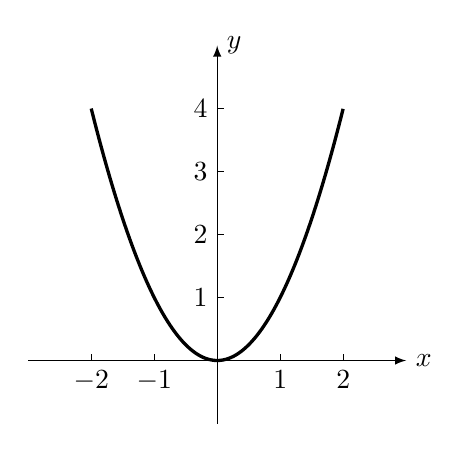
\begin{tikzpicture}[>=latex, scale=.8]
\draw[->](-3,0)--(3,0)node[right]{$x$};
\draw[->](0,-1)--(0,5)node[right]{$y$};
\foreach \x in {-2,-1,1,2}
{
    \draw (\x,0)node[below]{$\x$}--(\x, 0.1);
}
\foreach \x in {1,2,...,4}
{
    \draw (0,\x)node[left]{$\x$}--(.1,\x);
}

\draw[domain=-2:2, samples=100, very thick] plot(\x,{\x*\x});

\end{tikzpicture}
    \caption{}
\end{figure}


从上面表格中可以看到这个函数有一个特点:当自变量
取绝对值相等而符号相反的两个值时(如$x$取1.5和$-1.5$),
它们对应的函数值相等($y$都取2.25),这说明$y$轴垂直平分以
点$(x,f(x))$, $(-x,f(-x))$为端点的线段,换句话说,点
$(x,f(x))$, $(-x,f(x))$是关于$y$轴对称的,因此抛物线$y=x^2$
是关于$y$轴对称的。

我们把具有这种特征
的函数叫做偶函数。$f(x)$
是偶函数的标志是:当自
变量$x$取一对互为相反
数的值时,函数的值不
变,就有$f(x)=f(-x)$。

一般地说,对于函数
$f(x)$, 设$x$和$-x$都属于函
数的定义域,如果
\[f(-x)=f(x)\]
那么函数$f(x)$叫做\textbf{偶函数},偶函数的图象关于$y$轴对称。

我们再来画函数$y=\frac{1}{8}x^3$的图象

先作出下面的数值表:
\begin{center}
\begin{tabular}{c|ccccccccccc}
    \hline
    $x$ &$\cdots$&$-4$&$-3$&$-2$&$-1$&0&1&2&3&4&$\cdots$\\
\hline
$y$ &$\cdots$&$-8$&$-3\frac{3}{8}$&$-1$&$-\frac{1}{8}$&0&$\frac{1}{8}$&1&$3\frac{3}{8}$&8&$\cdots$\\
\hline
\end{tabular}
\end{center}

根据表里这些对应值,作出函数$y=x^3$的图象如图
5.2。这个图象称为立方抛物线。
\begin{figure}[htp]
    \centering
\begin{tikzpicture}[>=latex, scale=.5]
\draw[->](-5,0)--(5,0)node[right]{$x$};
\draw[->](0,-9)--(0,9)node[right]{$y$};
\foreach \x in {1,2,3,4}
{
    \draw (\x,0)node[below]{$\x$}--(\x, 0.1);
}
\foreach \x in {-2,-4}
{
    \draw (\x,0)node[above]{$\x$}--(\x, -0.1);
}
\foreach \x in {-8,-6,...,-2,2,4,...,8}
{
    \draw (0,\x)node[left]{$\x$}--(0.1,\x);
}
\node at (-.5,-.5){$O$};
\draw[domain=-4:4, samples=100, very thick] plot(\x,{\x*\x*\x/8});

\end{tikzpicture}
    \caption{}
\end{figure}

从上面表格中可以看到这个函数也有一个特征:因为,
$\frac{1}{8}(-x)^3=-\frac{1}{8}x^3$, 所以当自变量取两个互为相反数的值时,
对应的函数值也是互为相反数。所以如果点$(x,f(x))$在函
数的图象上,那么必有另一点$(-x,-f(x))$也在函数的图象
上,而原点恰是以$(x,f(x))$, $(-x,-f(x))$为端点的线段
的中点,换句话说,点$(x,f(x))$, $(-x,-f(x))$是关于原
点对称的。因此立方抛物线
$y=\frac{1}{8}x^3$是关于原点对称的,我
们把具有这种特征的函数叫做
奇函数,$f(x)$是奇函数的标志
是:当自变量$x$取一对互为相
反数的值时,函数的值也是
互为相反数,就是$f(-x)=-f(x)$。

一般地说,对于函数$f(x)$, 设$x$与$-x$都属于函数的定义
域,如果$$f(-x)=-f(x)$$ 那么函数$f(x)$叫做\textbf{奇函数}。奇函数的图象关于原点对称。

考虑一个函数是偶函数、奇函数,或者既不是偶函数又
不是奇函数,叫做研究函数的奇偶性,对于一个奇函数或者
偶函数,要了解它的性质和图象,只要了解当自变量取正
值时的性质和图象就可以了。例如,要作函数$y=\frac{1}{8}x^3$的图
象,因为它是奇函数,所以只要作出自变量取正值时的函数
图象,就可以利用奇函数的图象必定关于原点对称这一特点,
作出自变量取负值时的图象。

\begin{example}
研究下列函数的奇偶性:
\[f(x)=x^4+x^2,\qquad f(x)=x^3+x,\qquad f(x)=x+1\]   
\end{example}

\begin{solution}
\begin{enumerate}
    \item 对于$f(x)=x^4+x^2$, 我们有:
    \[f(-x)=(-x)^4+(-x)^2=x^4+x^2=f(x)\]
    $\therefore\quad $函数$f(x)=x^4+x^2$是偶函数。
    \item 对于$f(x)=x^3+x$, 我们有:
    \[f(-x)=(-x)^3+(-x)=-(x^3+x)=-f(x)\]
    $\therefore\quad $函数$f(x)=x^3+x$是奇函数。
    \item 对于$f(x)=x+1$, 我们有:
    \[f(-x)=-x+1\]
    这里$f(-x)\ne f(x)$, 并且$f(-x)\ne -f(x)$, 所以函数$f(x)=
x+1$既不是偶函数又不是奇函数。
\end{enumerate} 
\end{solution}

\begin{ex}
\begin{enumerate}
    \item  研究下面函数的奇偶性:(其中$k,b$是常数)
\begin{multicols}{2}
\begin{enumerate}
    \item $y=kx\quad (k\ne 0)$
    \item $y=\frac{k}{x}\quad (k\ne 0)$
    \item $y=kx+b\quad (k\ne 0)$
    \item $y=\sqrt{1+x^2}$
    \item $y=|x|$
    \item $y=\sqrt[3]{x}$
    \item $y=\sqrt{x}+1$
    \item $y=x^2+x+1$
\end{enumerate}
\end{multicols}
\item 证明:
\begin{enumerate}
    \item 两个偶函数的和是偶函数;
    \item 两个奇函数的和是奇函数;
    \item 两个偶函数的乘积是偶函数,
    \item 两个奇函数的乘积是偶函数;
    \item 偶函数与奇函数的乘积是奇函数。
\end{enumerate}
\end{enumerate}
\end{ex}

\subsection{函数$y=ax^2\; (a\ne 0)$的图象和性质}
在上一章里,我们研究了$x$的一次函数$y=ax+b$, 现在
我们要研究另一类重要的函数,这类函数的解析式是$x$的二
次式,我们把它叫做$x$的二次函数。

先看几个实例:

\begin{example}
    一石块离地面高为$h$, 设其速度为零,自由地落
到地面,运动的时间为$t$, 如果不考虑空气的阻力,于是$h$与
$t$之间将有函数关系:
\begin{equation}
 h=\frac{1}{2}gt^2   
\end{equation}
这里$g$是重力加速度。
\end{example}

\begin{example}
    农机厂第一个月水泵的产量为50(台),第三个月
的产量为$y$(台),与月平均增长
率之间的关系是:$y=50(1+x)^2$,即:
\begin{equation}
  y=50x^2+100x+50  
\end{equation}
\end{example}

\begin{example}
    设在半径是20厘米的
圆面上,从中心挖去一个半径为$x$厘米的圆面(图5.3),剩下的圆
环面积是$y$平方厘米,那么变量$y$和$x$间有下面的函数关系:
\begin{equation}
    y=400\pi-\pi x^2
\end{equation}
\end{example}

\begin{figure}[htp]
    \centering
\begin{tikzpicture}[>=latex]
 \draw [pattern=north east lines] (0,0) circle (1.5);
    \draw (0,0)[fill=white] circle (1);
\draw[->] (0,0)node[below]{$O$}--node[left]{$x$}(45:1);
\draw (0,0) -- (15:1.5);
\end{tikzpicture}    
    \caption{}
\end{figure}

从上面这些例子可以看出,它们有一个共同特点,那就
是每一个函数关系中,等号右边都是自变量的二次式。这些
函数都可以用
\begin{equation}
    y=ax^2+bx+c
\end{equation}
来表示,这里$a$是不等于零的实数,$b,c$是任意实数。

我们把函数$y=ax^2+bx+c\; (a\ne 0)$叫做$x$的二次函数。
下面我们先从最简单的情况开始研究,即研究在(5.4)中
取$b=0,c=0$的二次函数$y=ax^2\; (a\ne 0)$。

先来看$a>0$的情形。

我们已经在上一节和第三章中画过$y=x^2$和$y=\frac{1}{2}x^2$的图
象,现在把这两个图象和$y=2x^2$的图象都画在同一个坐标系
里。

先作下面的表:
\begin{center}
\begin{tabular}{c|ccccccccc}
    \hline
$x$ &$\cdots$ & $-2$  & $-\frac{3}{2}$  & $-1$   & 0   & 1&$\frac{3}{2}$& 2&$\cdots$\\
\hline
$y=2x^2$ &$\cdots$ & 8&$\frac{9}{2}$ &2  & 0   & 2&$\frac{9}{2}$ &8&$\cdots$\\
$y=x^2$ &$\cdots$ & 4&$\frac{9}{4}$&1  & 0   & 1&$\frac{9}{4}$&4&$\cdots$\\
$y=\frac{1}{2}x^2$ &$\cdots$ & $\frac{9}{8}$&$\frac{1}{2}$  & 0   & $\frac{1}{2}$  & $\frac{9}{8}$&2&$\cdots$\\
\hline
\end{tabular}    
\end{center}

\begin{figure}[htp]
    \centering
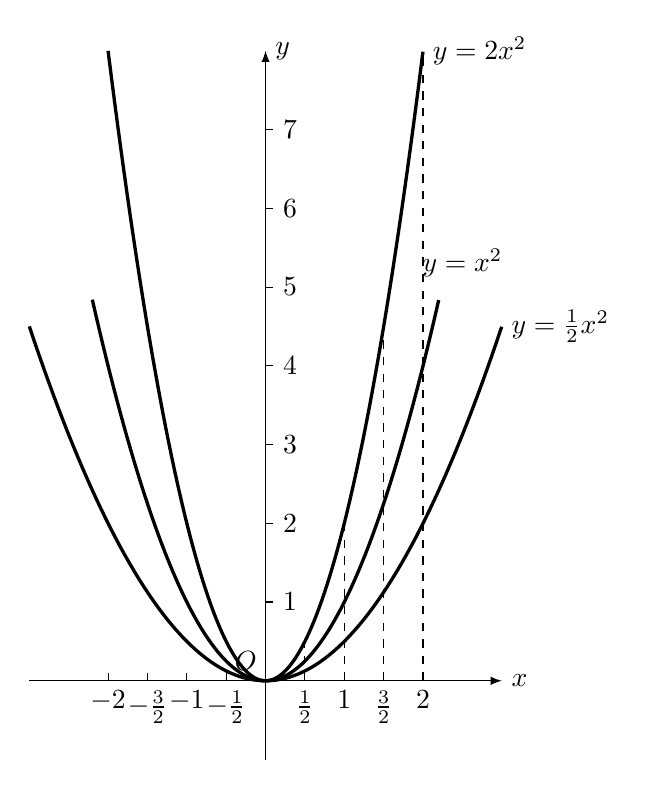
\begin{tikzpicture}[>=latex]
    \draw[->] (-3,0)--(3,0)node[right]{$x$};
    \draw [->] (0,-1)--(0,8)node[right]{$y$};
\foreach \y in {1,2,...,7}
{
    \draw (0,\y)--(.1,\y)node[right]{$\y$};
}
\foreach \x/\xtext in {-4/-2,-3/-\frac{3}{2},-2/-1,-1/-\frac{1}{2},1/\frac{1}{2},2/1,3/\frac{3}{2},4/2}
{
    \draw (\x/2,0)node[below]{$\xtext$}--(\x/2,.1);
}

\draw [domain=-3:3, samples=100, very thick]plot(\x,{\x*\x*0.5});
\draw [domain=-2.2:2.2, samples=100, very thick]plot(\x,{\x*\x});
\draw [domain=-2:2, samples=100, very thick]plot(\x,{\x*\x*2});
\node at (-.25,.25){$O$};
\foreach \x in {.5,1,...,2}
{
    \draw[dashed] (\x,0)--(\x,2*\x*\x);
}
\node at (2,8)[right]{$y=2x^2$};
\node at (2.5,5)[above]{$y=x^2$};
\node at (3,4.5)[right]{$y=\frac{1}{2}x^2$};
\end{tikzpicture}
    \caption{}
\end{figure}

从这个表可以看到,对于同一个$x$值,函数$y=2x^2$所对应
的值是函数$y=x^2$所对应的值的2倍。所以要画出函数$y=2x^2$
的图象,可以用$y=x^2$的图象为基础。

除了让这图象上的原点不动外,其它每一点的纵坐标都
拉长到原来的2倍,这样得到的新的点集就是$y=2x^2$的图象。
作图时我们只描出图象上几个关于$y$轴对称的点,如上表所
示,然后用平滑的曲线把它们连接起来。

同理,要作出函数$y=\frac{1}{2}x^2$的图象,也可以用$y=x^2$的图
象为基础。除了让$y=x^2$的图象上的原点不动外,其它每一点
的纵标都压缩到原来的$\frac{1}{2}$,便得到$y=\frac{1}{2}x^2$的图象。作图时
我们只描出图象上关于$y$轴对称的点,如上表所示,然后用
平滑曲线把它们连接起来。这样,就得到这三个函数的图象如图5.4。

再来看$a<0$的情形:

例如,我们要画函数$y=-x^2$的图象,也可以在函数$y=x^2$
的图象的基础上来研究。

作下面的表:
\begin{center}
\begin{tabular}{c|ccccccccc}
    \hline
$x$ &$\cdots$ & $-2$  & $-\frac{3}{2}$  & $-1$   & 0   & 1&$\frac{3}{2}$& 2&$\cdots$\\
\hline
$y=x^2$ &$\cdots$ & 4&$\frac{9}{4}$&1  & 0   & 1&$\frac{9}{4}$&4&$\cdots$\\
$y=-x^2$ &$\cdots$ & $-4$&$-\frac{9}{4}$&$-1$  & 0   & $-1$&$-\frac{9}{4}$&$-4$&$\cdots$\\
\hline
\end{tabular}    
\end{center}

从这个表可以看到,对于同一个$x$值,函数$y=-x^2$所对
应的值,恰巧是函数$y=x^2$所对应的值的相反数,当$x$遍取一
切实数值时,把函数$y=x^2$图象上的每一点纵坐标改为它的
相反数就得到函数$y=-x^2$的图象上的点,而以$(x,-x^2)$和
$(x,x^2)$为坐标的点是关于$x$轴的对称点,因此把图象$y=x^2$沿
$x$轴折转过来就可以得到$y=-x^2$的图象.$y=-x^2$的图象是在
$x$轴下方,开口向下(图5.5)。

同样,从函数$y=2x^2$和$y=4x^2$的图象可得出函数$y=
-2x^2$和$y=-4x^2$的图象(图5.6)。这些图象在x轴下方,开
口向下。

\begin{figure}[htp]\centering
    \begin{minipage}[t]{0.48\textwidth}
    \centering
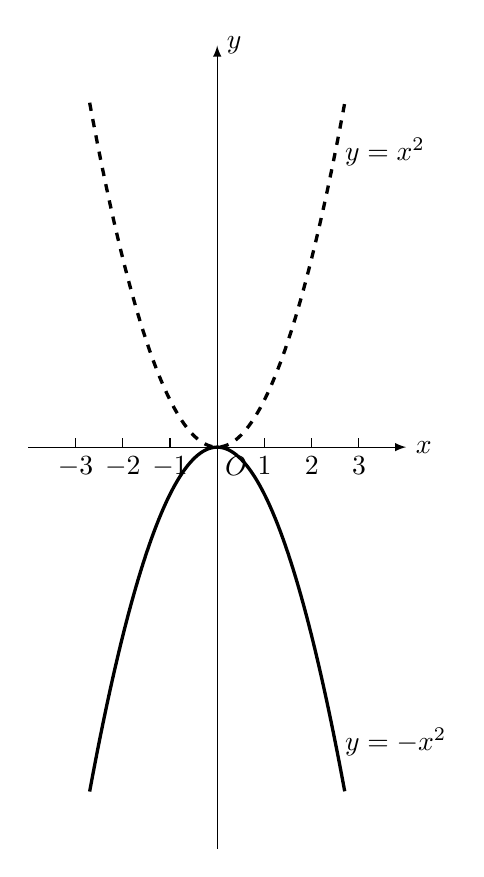
\begin{tikzpicture}[>=latex, scale=.6]
      \draw[->] (-4,0)--(4,0)node[right]{$x$};
    \draw [->] (0,-8.5)--(0,8.5)node[right]{$y$};

\foreach \x in {-3,-2,-1,1,2,3}
{
    \draw (\x,0)node[below]{$\x$}--(\x,.2);
}

\draw [domain=-2.7:2.7, samples=100, dashed, very thick]plot(\x,{\x*\x});
\draw [domain=-2.7:2.7, samples=100, very thick]plot(\x,{-\x*\x});
\node at (.4,-.4){$O$};
\node at (2.5,6.25)[right]{$y=x^2$};
\node at (2.5,-6.25)[right]{$y=-x^2$}; 
    \end{tikzpicture}
    \caption{}
    \end{minipage}
    \begin{minipage}[t]{0.48\textwidth}
    \centering
    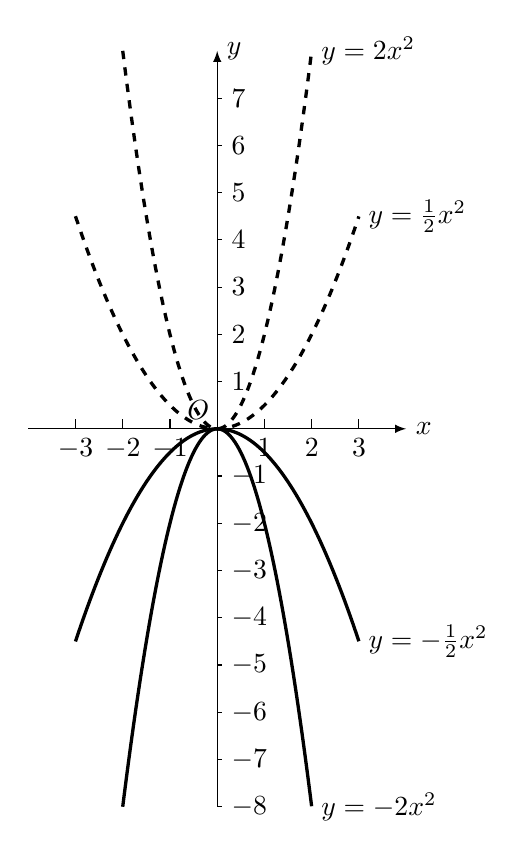
\begin{tikzpicture}[>=latex, scale=.6]
\draw[->] (-4,0)--(4,0)node[right]{$x$};
    \draw [->] (0,-8)--(0,8)node[right]{$y$};
\foreach \y in {-8,-7,...,-1,1,2,...,7}
{
    \draw (0,\y)--(.1,\y)node[right]{$\y$};
}
\foreach \x in {-3,-2,-1,1,2,3}
{
    \draw (\x,0)node[below]{$\x$}--(\x,.2);
}

\draw [domain=-3:3, samples=100, very thick, dashed]plot(\x,{\x*\x*0.5});
\draw [domain=-2:2, samples=100, very thick, dashed]plot(\x,{\x*\x*2});

\draw [domain=-3:3, samples=100, very thick]plot(\x,{-\x*\x*0.5});
\draw [domain=-2:2, samples=100, very thick]plot(\x,{-\x*\x*2});
\node at (-.4,.4){$O$};
\node at (2,8)[right]{$y=2x^2$};
\node at (3,4.5)[right]{$y=\frac{1}{2}x^2$};
\node at (2,-8)[right]{$y=-2x^2$};
\node at (3,-4.5)[right]{$y=-\frac{1}{2}x^2$};      
    \end{tikzpicture}
    \caption{}
    \end{minipage}
    \end{figure}

总结上面这两种情况,我们知道函数$y=ax^2$的图象是一
条抛物线。

从图象上我们能看到二次函数$y=ax^2$的下面一些性质:
\begin{enumerate}
    \item 抛物线$y=ax^2$可向$x$轴左右方向无限延伸。这就是说
函数$y=ax^2$的定义域为实数集$\mathbb{R}$.
\item 抛物线$y=ax^2$在$a>0$时,在$x$轴上方且在$y$轴的左
右两侧同时向上无限延伸,这就是说函数$y=ax^2$在$a>0$时,
函数值域为非负实数,即$\mathbb{R}^{+}\cup \{0\}$; 在$a<0$时,抛物线
$y=ax^2$在$x$轴下方且在y轴两侧同时向下无限延伸,这就是说
函数$y=ax^2$在$a<0$时,函数值域为非正实数,即$\mathbb{R}^{-}\cup \{0\}$.
\item 抛物线$y=ax^2$在$a>0$时开口向上,在$a<0$时开口
向下,且$|a|$越大开口就越小。
\item 抛物线$y=ax^2$关于$y$轴对称,这就是说函数$y=ax^2$是
个偶函数,事实上这个性质是可以证明的,即由于$f(-x)=
a(-x)^2=ax^2=f(x)$, 故函数$y=ax^2$是个偶函数.我们把$y$轴称
为抛物线$y=ax^2$的对称轴,其方程是$x=0$。
\item 抛物线$y=ax^2$当$a>0$时,图象在$(-\infty,0)$是下
降的,在$(0,+\infty)$是上升的。这就是说函数$y=ax^2$当$a>0$
时,在$(-\infty,0)$是递减的;在$(0,+\infty)$是递增的(图5.7)。

抛物线$y=ax^2$当$a<0$时,图象在$(-\infty,0)$是上升的,
在$(0,+\infty)$是下降的,这就是说函数$y=ax^2$当$a<0$时,
在$(-\infty,0)$是递增的;在$(0,+\infty)$是递减的(图5.8)。
\end{enumerate}

\begin{figure}[htp]\centering
    \begin{minipage}[t]{0.48\textwidth}
    \centering
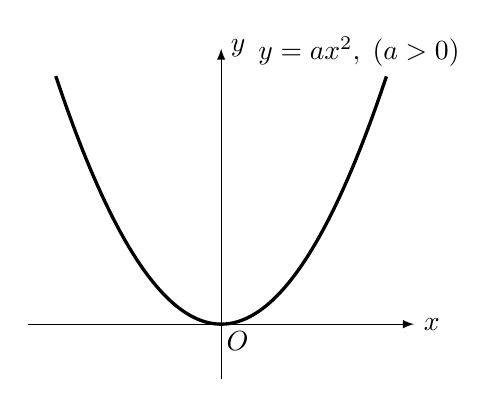
\begin{tikzpicture}[>=latex, scale=.7]
    \draw[->] (-3.5,0)--(3.5,0)node[right]{$x$};
    \draw [->] (0,-1)--(0,5)node[right]{$y$};
    \draw [domain=-3:3, samples=100, very thick]plot(\x,{\x*\x*0.5});
    \node at (2.5,4.5)[above]{$y=ax^2,\; (a>0)$};
    \node at (.3,-.3){$O$};
    \end{tikzpicture}
    \caption{}
    \end{minipage}
    \begin{minipage}[t]{0.48\textwidth}
    \centering
    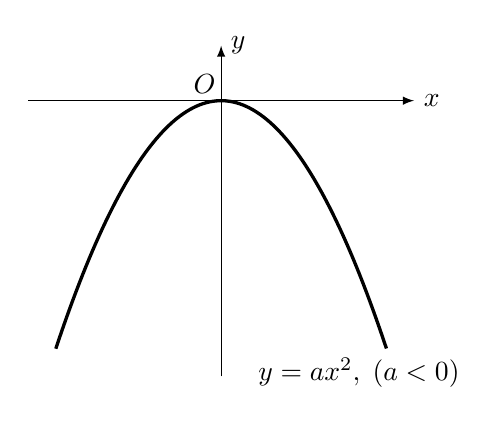
\begin{tikzpicture}[>=latex, scale=.7]
        \draw[->]  (-3.5,0)--(3.5,0)node[right]{$x$};
        \draw [->] (0,-5)--(0,1)node[right]{$y$};
        \draw [domain=-3:3, samples=100, very thick]plot(\x,{-\x*\x*0.5});    
    \node at (2.5,-4.5)[below]{$y=ax^2,\; (a<0)$};
    \node at (-.3,.3){$O$};
    \end{tikzpicture}
    \caption{}
    \end{minipage}
    \end{figure}

事实上,这个性质是可以证明的,我们只证$a>0$的情
况,$a<0$的情况留给同学们自己证明。









\begin{example}
    
\end{example}

\begin{example}
    
\end{example}



\begin{solution}
    
\end{solution}

\begin{solution}
    
\end{solution}


\begin{solution}
    
\end{solution}

\begin{solution}
    
\end{solution}


\begin{example}
    
\end{example}

\begin{solution}
    
\end{solution}

\begin{solution}
    
\end{solution}


\begin{example}
    
\end{example}

\begin{example}
    
\end{example}

\begin{example}
    
\end{example}




















\begin{example}
    
\end{example}

